\subsection{Localisation} 
As mentioned in Section~\ref{sec:comms} and in the literature review in Section~\ref{sec:lit}, localisation for this project relies on the Vicon Positioning System. The use of PyVicon, the Vicon SDK, and MAVProxy has already been discussed. In this section, the focus shifts to the coordinate‑system transformation and ArduPilot compatibility.

To begin, recall that the Vicon Positioning System, after processing through the GCS, outputs positional data in the form of GPS coordinates. These coordinates are mapped from the indoor flight arena (the testing environment) to the global map coordinate system. Each coordinate system has its own origin, defined as $(0,0)$. In the Geographic Coordinate System, this corresponds to a point west of Gabon, Africa, where both longitude and latitude equal zero. In contrast, the Vicon coordinate system defines its origin relative to the placement of the calibration wand during the Vicon calibration procedure.

To integrate the Vicon environment with the Pixhawk flight controller, which uses the Geographic Coordinate System, a coordinate transformation is required. A transformation is developed by aligning the origins of both systems, along with their respective axes. Once the relationship between Vicon’s local coordinate frame and the transformed GPS coordinates is established, a unified coordinate system relative to the shared origin can be defined. Visually, this relationship is expressed as follows:
in figure \ref{fig:coordTransform} below:
\begin{figure}[H]
    \centering
    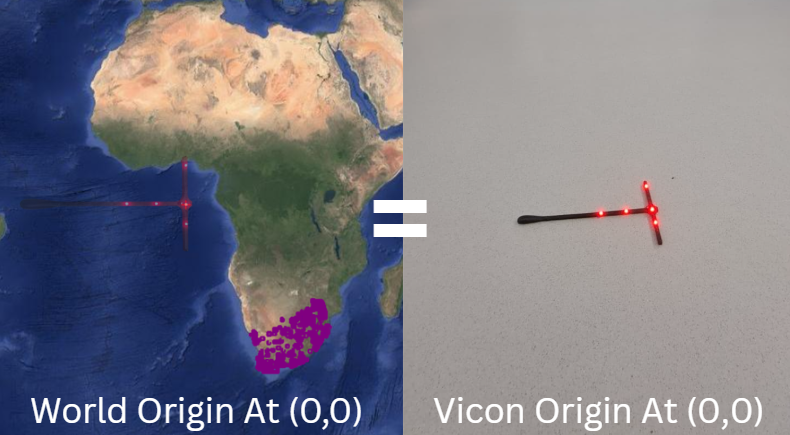
\includegraphics[width=0.8\linewidth]{Images/coord transfrom.png}
    \caption{Coordinate Transform between Vicon Origin and World Coordinates}
    \label{fig:coordTransform}
\end{figure}
Once a unified coordinate system is defined, MissionPlanner’s default path following features become fully usable. This also enables seamless integration across different subsystems, such as path planning and path following, as both can be developed using GPS formatted waypoints.

An automated mission can be created by manually placing the drone at each desired waypoint within the flight arena, where the corresponding coordinates must be recorded. These coordinates are then entered into MissionPlanner’s Planner interface to command the drone to visit each waypoint. An example of this process is shown in Figure~\ref{fig:waypoints}.This process was used during inital mapping stages, before path-planning subsystem was fully integrated into the overall system. 

\begin{figure}[H]
    \centering
    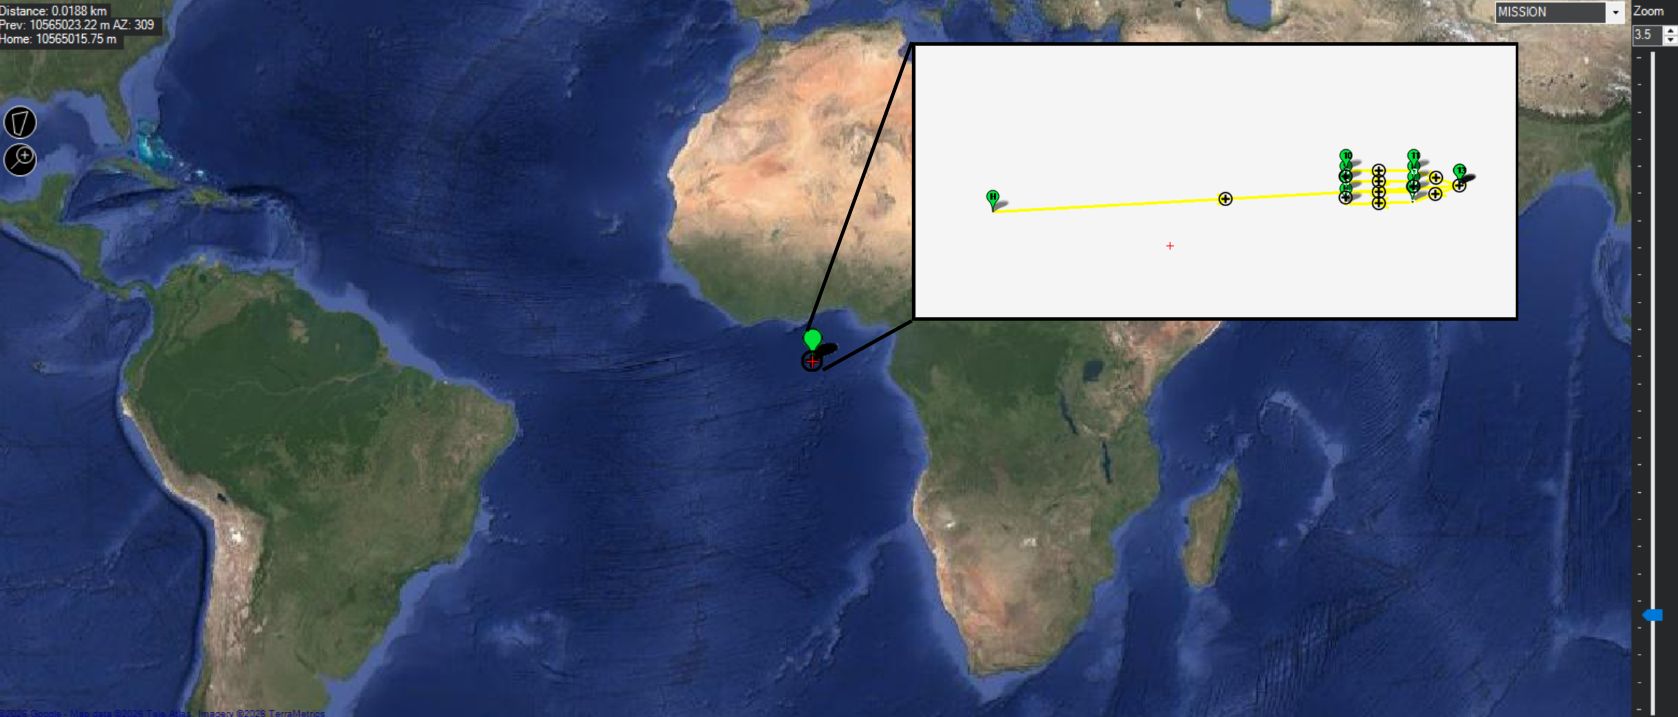
\includegraphics[width=0.8\linewidth]{Images/Waypoints.png}
    \caption{Example waypoints setup}
    \label{fig:waypoints}
\end{figure}

Once the coordinate system is defined, the next step is to ensure that the drone correctly interprets the newly implemented localisation method. This is achieved by disabling all onboard sensor sources within MissionPlanner, effectively removing the drone’s native spatial awareness inputs and forcing it to rely entirely on Vicon for localisation. This configuration is applied by modifying the EKF3 (Enhanced Kalman Filter) parameters. The following parameter settings ensure that EKF3 uses only the externally injected GPS data provided by the GCS as its sole positional input.

This subsystem is responsible for converting planned inspection targets into executable UAV motion commands. It provides the interface between the high-level planning modules and the low-level flight controller, enabling autonomous take-off, waypoint following, hovering, and landing.

The control implementation is based on MAVLink communication using \texttt{pymavlink}. A Python-based mission controller was developed to send position setpoints to the UAV in \texttt{GUIDED} mode. After establishing communication and receiving a heartbeat from the autopilot, the controller arms the vehicle, commands take-off to a predefined altitude, executes the mission by sending waypoint commands, and finally initiates landing.

Waypoint following is implemented by repeatedly transmitting local position targets in the \texttt{MAV\_FRAME\_LOCAL\_NED} frame. In this approach, the UAV is not given a full trajectory in advance; instead, the desired target position is sent continuously at a fixed rate. This ensures that the autopilot maintains the commanded position and allows stable hovering at inspection points.

For the surveyor UAV, a lawnmower coverage pattern is converted into an ordered list of waypoints. The mission begins by taking the UAV's post-takeoff position as a reference corner of the inspection area. Based on the specified room dimensions, lane spacing, and margin, a sequence of parallel sweep waypoints is generated. The UAV then transitions between these waypoints while maintaining constant altitude and fixed yaw.

To improve motion smoothness during transitions, intermediate position commands are generated using interpolation between consecutive waypoints. A smoothstep function is applied to reduce abrupt motion changes and produce more continuous movement. This is particularly beneficial for mapping, since it reduces aggressive manoeuvres that may degrade sensor measurements and map consistency.

For the inspector UAV, the execution strategy is simpler and goal-oriented. Once a feature of interest (FOI) has been identified in the map, its coordinates are transformed into the UAV local control frame and the vehicle is commanded directly from its current position to the target location. The UAV then hovers at the inspection position for a fixed duration before returning to its home position and landing.

A key design requirement is the transformation between the mapping frame and the local control frame used by the autopilot. The surveyor UAV produces a map in a local map coordinate system, while the autopilot executes commands in the MAVLink local NED frame. Since localisation is provided by the Vicon motion capture system rather than GNSS, the origin and orientation of the map must be aligned with the local frame before target coordinates can be executed. This is achieved by defining the map origin in local coordinates and applying a planar rotation and translation to convert map-frame FOI positions into local navigation targets.

In the final real-world implementation, motion execution for the inspector UAV was intentionally simplified to straight-line point-to-point navigation. Rather than executing a full obstacle-aware path, the UAV was commanded directly from the start position to the inspection target using a single linear segment. This simplification was appropriate because experiments were conducted in a controlled indoor environment with accurate Vicon-based localisation and no dynamic obstacles. The approach reduced implementation complexity while still demonstrating autonomous target reaching and inspection behaviour. \footnote{Nura Efendic}

Other then \texttt{GUIDED} mode for the mission controller the \texttt{AUTO} mode was also implemented for purpose of testing mapping before the path planning subsystem was finalized. Initially ArduPilot's Mission Planner waypoints were used \footnote{Cheuk Hei Matthew Tam}, which rely on the localisation system and predefined waypoints. This method requires prior knowledge of the room dimensions. 

% \begin{figure}[H]
%     \centering
%     \includegraphics[width=1\linewidth]{Images/Pathfollowing.png}
%     \caption{ ArduPilot's Mission Planner waypoints used for initial testing of the RTAB efficiency if UAV is performing CPP }
%     \label{fig:mission_planner}
% \end{figure}
However, this method was only used for the initial beginning phases of the project and later on the explained \texttt{GUIDED} mode was utilized and waypoint generating is based on the more generic approach and parameters as previously explained.